\subsection{Knochentypen}
Die 1038 Funde umfassen 14 verschiedene Knochentypen, welche in  \autoref{fig:horse_skeleton} \cite{WikiSkeletalHorse} übersichtlich dargestellt sind.
Da unterschiedliche Knochen unterschiedlich groß sind, ist ein Vergleich zwischen verschiedenen Knochentypen nicht sinnvoll. 
Stattdessen müssen die Daten nach den verschiedenen Knochentypen (Attribut \texttt{ELEMENT}) gruppiert und dann innerhalb dieser Gruppen untersucht werden.
Die Aufteilung in Gruppen nach Knochentyp geschieht in \texttt{an\_2}. 

\begin{figure}[H]
    \centering
    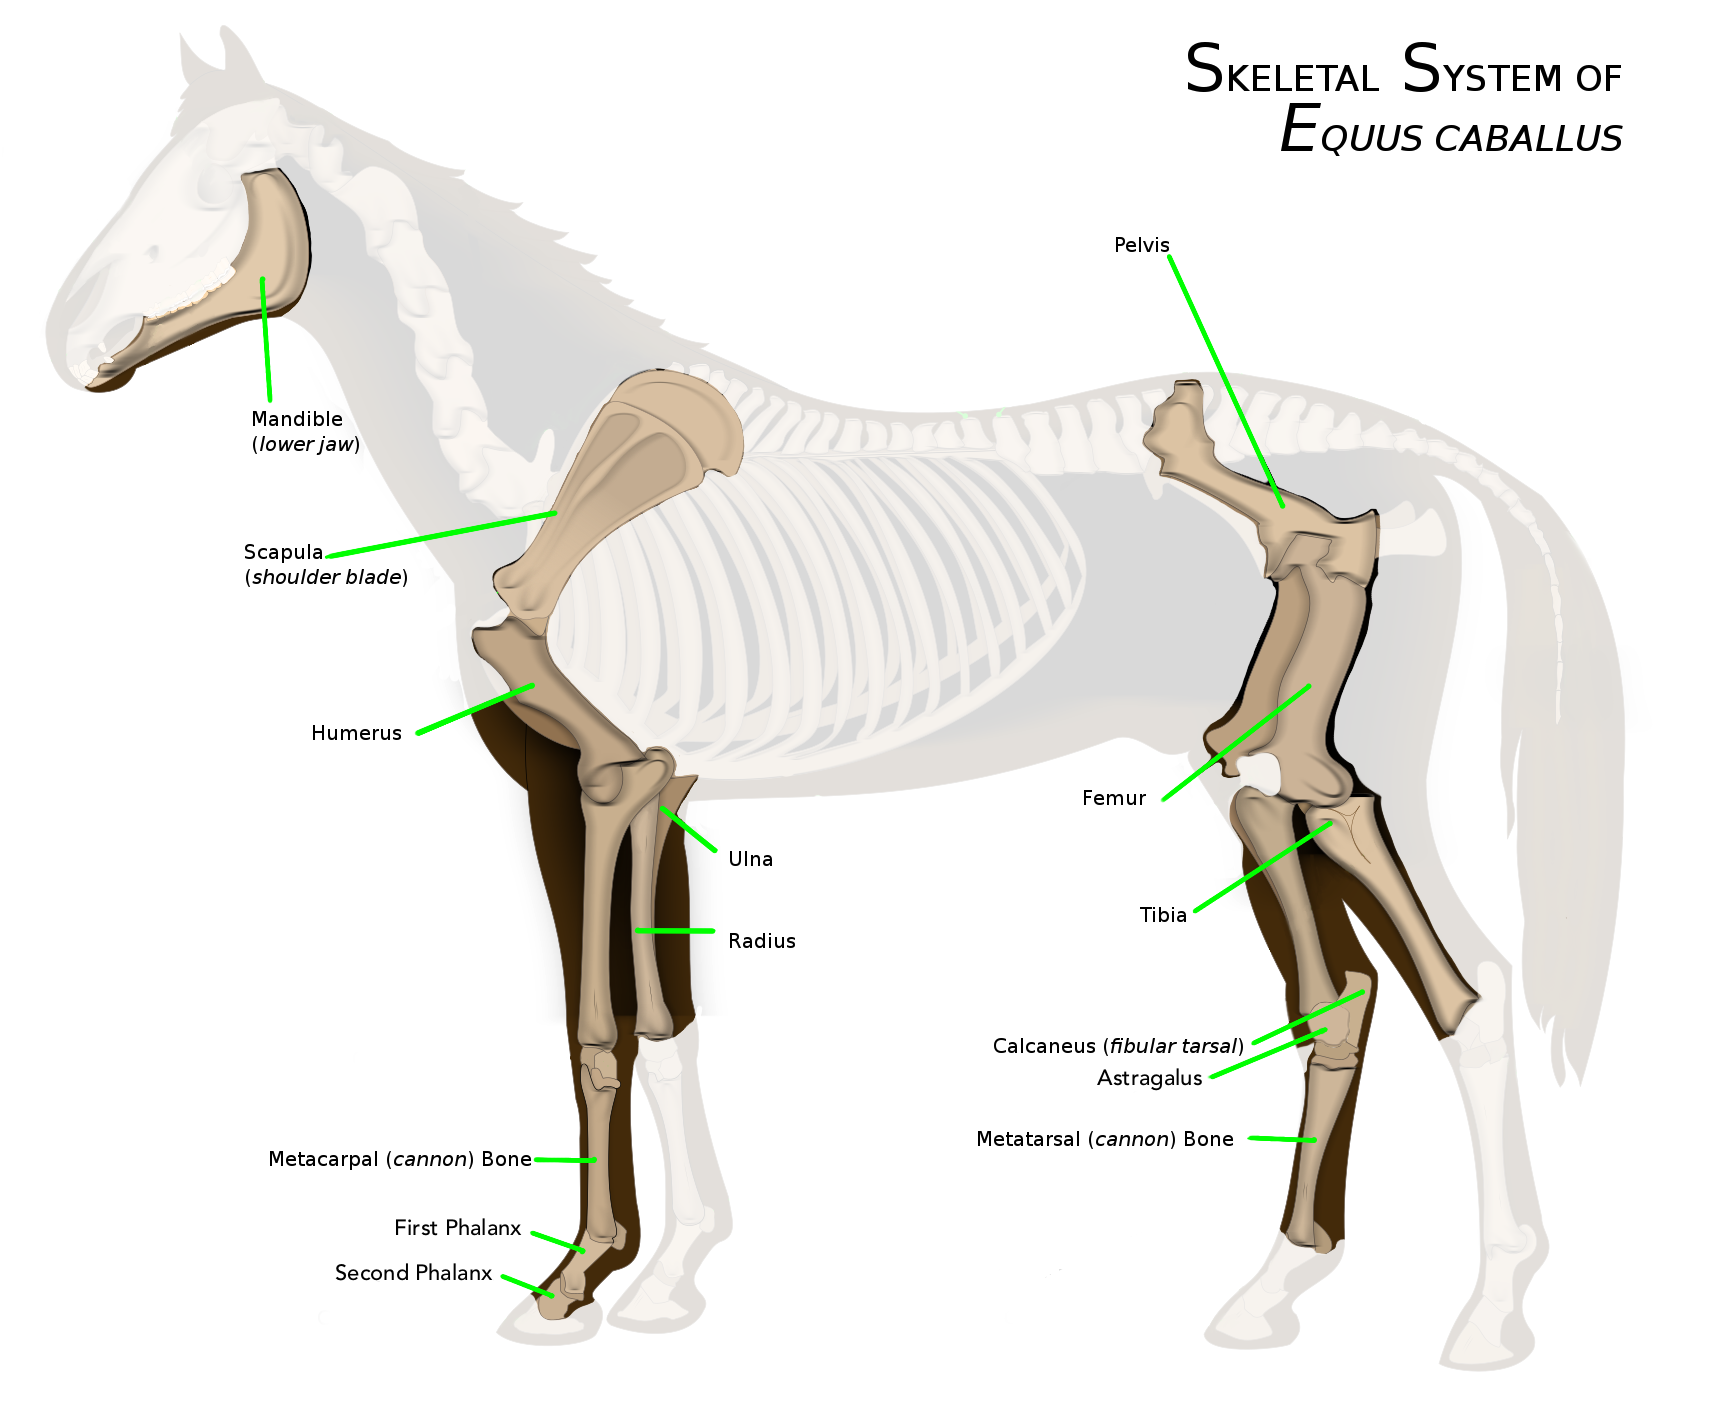
\includegraphics[height=10cm]{docs/attachments/ab-project_Horse-anatomy.png}
    \caption{Die im Datensatz vorhandenen Knochen sind beschriftet und farblich hervorgehoben}
    \label{fig:horse_skeleton}
\end{figure}

\autoref{fig:barchart} zeigt jeweils die Menge an Funden und Messungen pro Knochentyp.

\begin{figure}[H]
    \centering
    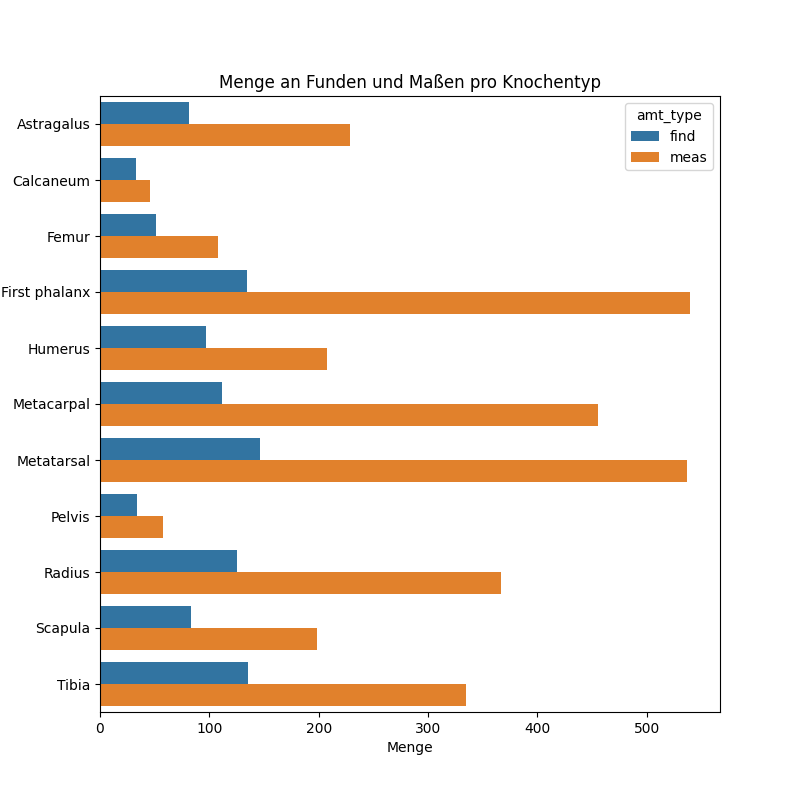
\includegraphics[height=10cm]{results/plots/amounts_barchart.png}
    \caption{Die Menge an Funden und Messungen pro Knochentyp}
    \label{fig:barchart}
\end{figure}
